\documentclass[11pt,letterpaper]{article}
\usepackage[provide=*,spanish]{babel}
\usepackage{fontspec}
\setmainfont{Latin Modern Roman}
\setsansfont{Latin Modern Sans}
\usepackage[margin=18mm,headheight=14pt,footskip=9mm]{geometry}
\usepackage{microtype,booktabs,array,tabularx,xcolor,graphicx,amsmath,hyperref,fancyhdr,tikz,float}
\usetikzlibrary{arrows.meta,positioning,shapes.geometric}
\definecolor{navy}{HTML}{14324C}
\definecolor{teal}{HTML}{008A89}
\definecolor{pale}{HTML}{EDF5F5}
\definecolor{amber}{HTML}{D88E26}
\hypersetup{colorlinks=true,linkcolor=navy,urlcolor=teal}
\pagestyle{fancy}
\fancyhf{}
\lhead{\sffamily\small UTEC · Planificación y Toma de Decisiones en IA}
\rhead{\sffamily\small Proyecto 1 · IEEE-CIS}
\cfoot{\sffamily\small\thepage}
\renewcommand{\headrulewidth}{.35pt}
\setlength{\parindent}{0pt}
\setlength{\parskip}{3.5pt}
\linespread{1.03}
\renewcommand{\arraystretch}{1.11}
\newcommand{\aparef}[1]{\par\hangindent=1.2em\hangafter=1 #1\par}

\begin{document}

\begin{center}
{\Large\sffamily\bfseries\color{navy} Sistema adaptativo de detección de fraude}\\[2pt]
{\large\sffamily Decisiones bajo datos no estacionarios en IEEE-CIS}\\[6pt]
{\small Departamento de Ciencia de la Computación · Proyecto 1 · 2026-1}\\[3pt]
{\small Equipo: \underline{\hspace{8cm}} \quad Fecha: \underline{\hspace{2.1cm}}}
\end{center}
\vspace{-4pt}\hrule\vspace{4pt}

\textbf{Resumen.} Se diseña y evalúa un sistema inteligente adaptativo para detección de fraude financiero con datos temporales. El sistema integra transacciones e identidad, estima un score con un modelo LightGBM, traduce el score en acciones operativas y propone monitoreo de drift, calibración y reentrenamiento con ventanas deslizantes. Los resultados provienen de los artefactos V01--V06 del repositorio: EDA propio, kernels de Kaggle, reportes y CSV de métricas. La recomendación final es usar V01 como modelo base, V05 como política inicial y V06 como soporte de robustez/calibración.

\section{Problema, objetivos y restricciones}

El conjunto IEEE-CIS Fraud Detection contiene transacciones electrónicas y atributos de identidad unidos por \texttt{TransactionID}. El caso de uso es clasificar transacciones futuras como riesgo bajo, riesgo intermedio o riesgo alto, para decidir si se aprueban, se envían a revisión humana o se escalan. El problema es no estacionario: la tasa de fraude y la distribución de variables cambian en el tiempo. En la literatura, este fenómeno se asocia a \emph{concept drift}, es decir, cambios temporales en la relación entre entradas y salida (Gama et al., 2014).

\begin{table}[H]\centering\small
\begin{tabularx}{\linewidth}{@{}p{.23\linewidth}X X@{}}\toprule
Objetivo & Métrica & Restricción o riesgo\\\midrule
Detectar fraude & PR-AUC, ROC-AUC, recall por ventana & Clase positiva minoritaria; no usar accuracy como criterio central.\\
Decidir con capacidad limitada & Costo normalizado, fraude capturado, revisión, escalamiento & Capacidad objetivo de revisión cercana a 5\%.\\
Controlar incertidumbre & Brier, calibración, estabilidad del score & No comunicar score bruto como probabilidad sin calibración.\\
Monitorear drift & KS, PSI, missingness, métricas por ventana & No asumir que el entrenamiento representa indefinidamente al futuro.\\
Reducir fricción social & Legítimas escaladas, UID conocido/desconocido & Evitar automatizar casos ambiguos sin revisión humana.\\\bottomrule
\end{tabularx}
\end{table}

La métrica principal de modelado es PR-AUC porque el fraude representa sólo 3.50\% del entrenamiento; en datos desbalanceados, las curvas Precision-Recall son más informativas que ROC o accuracy para evaluar la clase minoritaria (Saito \& Rehmsmeier, 2015). ROC-AUC se reporta como complemento.

\section{Análisis y preparación temporal}

El EDA propio reporta 590\,540 transacciones etiquetadas, 506\,691 registros de competencia sin etiqueta, 3.499\% de fraude en entrenamiento, 74 variables con más de 80\% de faltantes y tasa semanal de fraude entre 1.85\% y 5.06\%. Además, la validación adversarial train/test alcanzó ROC-AUC 1.000, señal de cambio observable entre periodos. Esto exige validación cronológica y evita tratar el problema como i.i.d.

\begin{center}
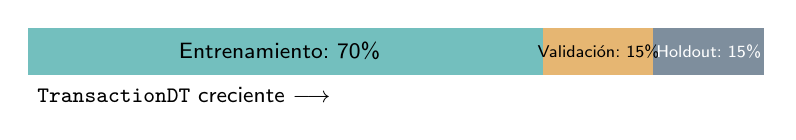
\begin{tikzpicture}[font=\sffamily\footnotesize,x=1cm,y=1cm]
\fill[navy!12] (0,0) rectangle (9.35,.6);
\fill[teal!55] (0,0) rectangle (6.545,.6);
\fill[amber!65] (6.545,0) rectangle (7.9475,.6);
\fill[navy!55] (7.9475,0) rectangle (9.35,.6);
\node at (3.2,.3){Entrenamiento: 70\%};
\node[scale=.77] at (7.25,.3){Validación: 15\%};
\node[scale=.77,text=white] at (8.65,.3){Holdout: 15\%};
\node[anchor=west] at (0,-.25){\texttt{TransactionDT} creciente $\longrightarrow$};
\end{tikzpicture}
\end{center}

Las transacciones se ordenan por \texttt{TransactionDT}. Los primeros 70\% se usan para entrenamiento, el 15\% siguiente para validación y el 15\% final como holdout futuro. \texttt{TransactionDT}, \texttt{DT\_day\_index} y \texttt{DT\_week\_index} no se usan como predictores porque codifican posición temporal absoluta; se reservan para partición y monitoreo. Las agregaciones por UID se consideran válidas sólo si usan información disponible antes de la transacción evaluada.

\section{Modelado y evaluación temporal}

La línea base V01 usa LightGBM con 185 atributos y \emph{early stopping}. La selección se justifica por la naturaleza tabular del dataset: variables numéricas, categóricas codificadas, faltantes e interacciones no lineales. Posteriormente se ejecutaron controles: V01b con todas las features, V02 con features UID históricas, V03 de auditoría de variables y V04 con LightGBM, XGBoost y CatBoost sobre sets auditados.

\begin{table}[H]\centering\small
\begin{tabularx}{\linewidth}{@{}p{.13\linewidth}X p{.23\linewidth}p{.22\linewidth}@{}}\toprule
Versión & Objetivo & Resultado principal & Decisión\\\midrule
V01 & Baseline temporal LightGBM & Holdout PR-AUC 0.5436 & Modelo base.\\
V01b & Usar todas las features & Holdout PR-AUC 0.5303 & No reemplaza V01.\\
V02 & Features UID históricas & UID conocido mejora; UID desconocido empeora & No adoptar como modelo único.\\
V03 & Auditoría de importancia y drift & 44 keep, 9 monitor & Usar para monitoreo.\\
V04 & Comparar LightGBM/XGBoost/CatBoost & Ninguno supera V01 & Mantener V01.\\\bottomrule
\end{tabularx}
\end{table}

\begin{table}[H]\centering\small
\begin{tabular}{@{}lrrr@{}}\toprule
Evaluación V01 & Prevalencia & PR-AUC & ROC-AUC\\\midrule
Validación global & 3.43\% & 0.5954 & 0.9257\\
Holdout global & 3.48\% & 0.5436 & 0.9051\\
Holdout UID conocido & 1.93\% & 0.5159 & 0.9020\\
Holdout UID desconocido & 4.73\% & 0.5632 & 0.8933\\\bottomrule
\end{tabular}
\end{table}

La caída de PR-AUC entre validación y holdout es consistente con degradación temporal. V02 demuestra que el historial UID sí contiene señal: en holdout UID conocido, \texttt{uid\_freq\_amt} sube de 0.5946 a 0.6831; sin embargo, UID desconocido cae de 0.5458 a 0.5315. Por ello no se adopta como modelo único. V04 confirma que podar agresivamente features reduce señal: el mejor candidato auditado queda en 0.5131 de PR-AUC holdout, por debajo de V01.

\textbf{Nota sobre la rúbrica.} La implementación existente compara tres enfoques avanzados de boosting y varios conjuntos de variables. Para cubrir literalmente ``dos enfoques tradicionales y uno avanzado'', se recomienda agregar en el notebook final una regresión logística regularizada y un bosque aleatorio o HistGradientBoosting simple, usando el mismo split temporal. Esta acción es de bajo riesgo y cerraría completamente ese ítem formal.

\section{Arquitectura, incertidumbre y decisión}

\begin{figure}[H]\centering
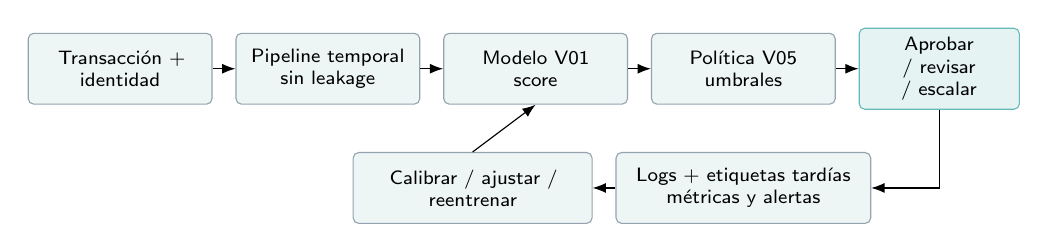
\begin{tikzpicture}[node distance=2.8mm and 2.9mm,>=Latex, font=\sffamily\scriptsize,
box/.style={draw=navy!45,rounded corners=2pt,align=center,text width=21mm,minimum height=9mm,fill=pale},
act/.style={draw=teal!60,rounded corners=2pt,align=center,text width=18mm,minimum height=9mm,fill=teal!10}]
\node[box] (data){Transacción +\\identidad};
\node[box,right=of data] (prep){Pipeline temporal\\sin leakage};
\node[box,right=of prep] (score){Modelo V01\\score};
\node[box,right=of score] (policy){Política V05\\umbrales};
\node[act,right=of policy] (action){Aprobar / revisar\\/ escalar};
\node[box,below=6mm of policy,text width=30mm] (mon){Logs + etiquetas tardías\\métricas y alertas};
\node[box,left=of mon,text width=28mm] (adapt){Calibrar / ajustar /\\reentrenar};
\draw[->] (data)--(prep);\draw[->] (prep)--(score);\draw[->] (score)--(policy);\draw[->] (policy)--(action);
\draw[->] (action.south) |- (mon.east);\draw[->] (mon)--(adapt);\draw[->] (adapt.north) -- (score.south);
\end{tikzpicture}
\caption{Arquitectura funcional propuesta para predicción, decisión y adaptación.}
\end{figure}

V06 muestra que el score bruto no debe interpretarse directamente como probabilidad: en holdout su promedio fue 14.30\% mientras la tasa real fue 3.48\%. La calibración isotónica redujo Brier de 0.0479 a 0.0219 y alineó el promedio calibrado a 3.55\%. Esto es coherente con la literatura: modelos fuertes pueden rankear bien pero producir probabilidades sesgadas, por lo que Platt scaling o isotonic regression son herramientas apropiadas para calibración (Niculescu-Mizil \& Caruana, 2005; Zadrozny \& Elkan, 2002).

\begin{table}[H]\centering\small
\begin{tabularx}{\linewidth}{@{}p{.18\linewidth}p{.22\linewidth}X@{}}\toprule
Acción & Regla V05 & Control de incertidumbre\\\midrule
Aprobar & $s<0.459783$ & Registrar decisión y permitir auditoría posterior.\\
Revisar & $0.459783\leq s<0.779122$ & Analista valida el caso y aporta etiqueta diferida.\\
Escalar & $s\geq0.779122$ & Bloqueo temporal o verificación adicional con revisión humana.\\\bottomrule
\end{tabularx}
\end{table}

En V05, los costos normalizados son 100 por fraude aprobado, 10 por legítima escalada y 2 por revisión manual. La política se selecciona en validación y se aplica a holdout sin recalibrar.

\begin{table}[H]\centering\small
\begin{tabular}{@{}lrrrr@{}}\toprule
Política en holdout & Costo/txn & Fraude detectado & Revisión & Escalamiento\\\midrule
Aprobar todo & 3.4804 & 0.00\% & 0.00\% & 0.00\%\\
Revisar top 5\% & 1.5247 & 59.20\% & 5.23\% & 0.00\%\\
Escalar top 1\% & 2.5959 & 25.75\% & 0.00\% & 1.01\%\\
V05 & \textbf{1.3680} & \textbf{66.17\%} & 5.10\% & 2.48\%\\\bottomrule
\end{tabular}
\end{table}

V05 supera a reglas simples, aunque la revisión en holdout (5.10\%) excede levemente el objetivo de 5\%. En producción, si el cupo fuera estricto, se recomienda usar umbrales por percentil temporal o una cola con capacidad fija.

\section{Despliegue y ciclo de vida}

La propuesta de despliegue sigue el taller de GCP: API, contenedor, Artifact Registry, Cloud Build y Cloud Run. La API \texttt{POST /predict} recibe una transacción, genera features, calcula score, aplica la política y retorna score, probabilidad calibrada opcional, decisión y versiones. Cloud Run es adecuado porque sirve contenedores HTTP, escala según demanda y se integra con Cloud Logging/Monitoring. Según la documentación oficial, Cloud Build puede construir la imagen, almacenarla en Artifact Registry y desplegarla en Cloud Run de forma automatizada.

\begin{table}[H]\centering\small
\begin{tabularx}{\linewidth}{@{}p{.26\linewidth}p{.22\linewidth}X@{}}\toprule
Elemento & Cadencia propuesta & Regla de cambio\\\midrule
Operación y cupo & Diario & Vigilar revisión, escalamiento, legítimas afectadas y latencia.\\
Desempeño con etiquetas & Semanal & PR-AUC, recall, Brier y costo por bloque y segmento.\\
Umbrales y calibración & Semanal / mensual & Ajustar sólo con datos anteriores a la ventana evaluada.\\
Modelo & Mensual o alerta sostenida & Comparar candidato frente al vigente en bloque futuro intocado.\\\bottomrule
\end{tabularx}
\end{table}

\section{Drift y adaptación}

La detección de drift combina señales inmediatas y señales con etiquetas tardías. Para numéricas se propone KS; para variables agrupadas o categóricas, PSI y cambios de missingness; para scores, percentiles y tasa sobre umbrales; para desempeño, PR-AUC, Brier, recall y costo por ventana. Las estrategias de olvido por ventanas deslizantes se apoyan en la idea de que datos antiguos pueden volverse menos relevantes cuando cambia el proceso generador (Bifet \& Gavalda, 2007).

\begin{table}[H]\centering\small
\begin{tabularx}{\linewidth}{@{}p{.22\linewidth}X X@{}}\toprule
Escenario por simular & Entrenamiento antes del bloque $t$ & Comparación en el bloque $t$\\\midrule
Sin olvido & Todo el historial disponible & Referencia de permanencia.\\
Ventana corta & Últimas 4 semanas etiquetadas & Reacción rápida; mayor varianza.\\
Ventana media & Últimas 8 semanas etiquetadas & Compromiso entre recencia y muestra.\\
Ventana larga & Últimas 12 semanas etiquetadas & Más estabilidad; posible lentitud.\\\bottomrule
\end{tabularx}
\end{table}

Cada iteración entrena con etiquetas disponibles antes de $t$, calibra en una subventana pasada, evalúa en el bloque futuro y agrega PR-AUC, recall, Brier, costo y métricas por UID. Un modelo nuevo sólo se promueve si mejora o iguala V01 en holdout temporal reciente, no empeora UID desconocido y respeta la capacidad operativa.

\section{Limitaciones y cierre}

Los costos son normalizados, no monetarios reales; el dataset está anonimizado; la equidad demográfica no puede auditarse directamente; y la política V05 excede levemente el cupo de revisión. Aun así, el proyecto cubre el ciclo de vida solicitado: definición del problema, EDA temporal, modelado, decisión, despliegue y adaptación. La recomendación final es V01 + V05 + monitoreo/calibración V06. El siguiente paso para cierre perfecto de rúbrica es ejecutar dos modelos tradicionales adicionales con el mismo split temporal y sumar sus métricas a la tabla comparativa.

\section*{Referencias}
\small
\aparef{Bifet, A., \& Gavalda, R. (2007). Learning from time-changing data with adaptive windowing. \emph{Proceedings of the SIAM International Conference on Data Mining}.}
\aparef{Gama, J., Zliobaite, I., Bifet, A., Pechenizkiy, M., \& Bouchachia, A. (2014). A survey on concept drift adaptation. \emph{ACM Computing Surveys, 46}(4), Article 44. https://doi.org/10.1145/2523813}
\aparef{Google Cloud. (2026). \emph{Deploying to Cloud Run using Cloud Build}. https://docs.cloud.google.com/build/docs/deploying-builds/deploy-cloud-run}
\aparef{Niculescu-Mizil, A., \& Caruana, R. (2005). Predicting good probabilities with supervised learning. \emph{Proceedings of the 22nd International Conference on Machine Learning}, 625--632. https://doi.org/10.1145/1102351.1102430}
\aparef{Saito, T., \& Rehmsmeier, M. (2015). The precision-recall plot is more informative than the ROC plot when evaluating binary classifiers on imbalanced datasets. \emph{PLOS ONE, 10}(3), e0118432. https://doi.org/10.1371/journal.pone.0118432}
\aparef{Zadrozny, B., \& Elkan, C. (2002). Transforming classifier scores into accurate multiclass probability estimates. \emph{Proceedings of the Eighth ACM SIGKDD International Conference on Knowledge Discovery and Data Mining}, 694--699. https://doi.org/10.1145/775047.775151}

\end{document}
